\documentclass[a4paper,12pt]{article}
\usepackage{titling}
\usepackage[OT4]{fontenc}
\usepackage[english,polish]{babel}
\usepackage{amsmath, amsfonts, amsthm, latexsym}

% Margins in document
\usepackage[left=2.5cm, right=2.5cm, top=3.5cm]{geometry}

% Indentation at the beginning of chapters/sections
\usepackage{indentfirst}

% Ceiling functions
\usepackage{mathtools}
\DeclarePairedDelimiter{\ceil}{\lceil}{\rceil}

% Avoid  colons before tables' empty captions and change caption
\usepackage{caption}
\captionsetup[table]{name=Tab.}
\captionsetup[figure]{name=Rys.}

% Don't know why, it starts from 2
\addtocounter{table}{0}

% Rename tables' suffix
\renewcommand{\tablename}{Tab.}

% Graphicx setup
\usepackage{graphicx}
\graphicspath{{graphics/}{../graphics/}}

\usepackage[table,x11names]{xcolor}

% No separator between items
\usepackage{enumitem}
\setlist{nolistsep}

% Pagebreak before every \section
\let\oldsection\section
\renewcommand\section{\clearpage\oldsection}

% Bigger padding in tabulars
\usepackage{array}
\setlength\extrarowheight{3pt}

% Itemize in tabulars (avoid big margins with minipage)
\newcommand{\tabbeditemize}[1]{
	\begin{minipage}[t]{0.4\textwidth}
		\begin{itemize}[topsep=0mm,partopsep=0mm,leftmargin=4mm]
			#1
		\end{itemize}
\end{minipage}}

% listings
\usepackage{xcolor}
\usepackage{listings}
\usepackage{hyperref}
\definecolor{codegreen}{rgb}{0,0.7,0}
\definecolor{codegray}{rgb}{0.5,0.5,0.5}
\definecolor{codepurple}{rgb}{0.58,0,0.82}
\definecolor{backcolour}{rgb}{0.95,0.95,0.92}
\lstdefinestyle{mystyle}{
	language=Python,
	deletekeywords={from},
	backgroundcolor=\color{backcolour},   
	commentstyle=\color{codegreen},
	keywordstyle=\color{magenta},
	numberstyle=\tiny\color{codegray},
	stringstyle=\color{codepurple},
	basicstyle=\ttfamily\footnotesize,
	breakatwhitespace=false,         
	breaklines=true,                 
	captionpos=b,                    
	keepspaces=true,                 
	numbers=left,                    
	numbersep=5pt,                  
	showspaces=false,                
	showstringspaces=false,
	showtabs=false,                  
	tabsize=4
}

% Nazwa gry
\newcommand{\nazwagry}{\textit{Connect4}}

%twopartdef
\newcommand{\twopartdef}[3]
{
	\left\{
	\begin{array}{ll}
		#1 & \mbox{jeśli agent wygrał} #2 \\
		#3 & \mbox{w p.p. } 
	\end{array}
	\right.
}

% DOCUMENT
\title{
	Zastosowanie algorytmu UCT do stworzenia sztucznej inteligencji grającej w \nazwagry\\
	\large Dokumentacja końcowa}

\author{Patryk Fijałkowski \\ Mateusz Burczaniuk}

% ============================================
% CONTENT ====================================
% ============================================

\begin{document}
\begin{titlingpage}
	\maketitle
	\vspace{3cm}
\end{titlingpage}

\section{Opis problemu}


\section{Sposób przeprowadzenia testów}
Każdy z przeprowadzonych testów będzie w formie pełnej rozgrywki \textit{Connect4} pomiędzy dwoma agentami. W celu oszacowania, jak dobre decyzje podejmował agent rozpoczynający rozgrywkę, zdefiniowano funkcję $REWARD$ opisaną równaniem (\ref{eq:reward}). Funkcja jest zależna od liczby ruchów $m$ w danej partii i przyjmuje wartości z zakresu $[-1; 0.8]$. Funkcja nie może przyjąć wartości większych od $0.8$ ze względu na przewagę pierwszego gracza spowodowaną faktem, że rozpoczyna on rozgrywkę.

\begin{equation} \label{eq:reward}
	REWARD(m) = \twopartdef { 0.8 \cdot (1 - \frac{m-7}{35}) } {} {\frac{m-7}{35} - 1}
\end{equation}



\section{Weryfikacja hipotez}
\subsection{Optymalne parametry}
W celu wyznaczenia najlepszych parametrów dla każdego z trzech analizowanych wariantów UCT, przeprowadzono rozgrywki z algorytmem heurystycznym. Dla każdego wariantu sprawdzono 20 próbnych konfiguracji parametrów, a każdą z konfiguracji sprawdzono dla 15 wartości ziarna generatora liczb losowych, by zmniejszyć wpływ losowości na działanie algorytmu. W każdym teście algorytm MCTS wykonywał 15.000 iteracji. Jako ocenę każdej konfiguracji przyjęto średnią arytmetyczną wartości funkcji $REWARD$ otrzymanych po zakończonych rozgrywkach. Wyniki testów ukazane są w tabelach \ref{tab:ucb1_param} - \ref{tab:ucbm_param}.

\begin{table}[!h]
	\centering
	\begin{tabular}{|c|c|} \hline
		Wartość $c$ & Ocena \\ \hline
		2 &	0.552 \\ \hline
		\rowcolor{teal} 1.41 &	0.529 \\ \hline
		1.7 &	0.484 \\ \hline
		1.6 &	0.425 \\ \hline
		1.5 &	0.415 \\ \hline
		1.45 &	0.401 \\ \hline
		1 &	0.153 \\ \hline
		0.09 &	-0.448 \\ \hline
		0.01 &	-0.563 \\ \hline
		0 & -0.702 \\ \hline
	\end{tabular}
	\caption{Ocena algorytmu UCB1 w zależności od parametru eksploracji}
	\label{tab:ucb1_param}
\end{table}

Jak widać w tabeli \ref{tab:ucb1_param}, algorytm UCB1 został najlepiej oceniony dla wartości parametru eksploracji $c=2$. Wraz ze zwiększaniem i zmniejszaniem wartości parametru, algorytm był oceniany gorzej. Ponadto, w przypadku $c=0$, kiedy algorytm eksploatował jedynie najbardziej obiecujące ruchy, podejmował najgorsze decyzje. Wartość sugerowana przez autorów algorytmu w \cite{banditbased} ($c=1.41$) została oceniona nieznacznie gorzej względem $c=2$.

\clearpage

\begin{table}[!h]
	\centering
	\begin{tabular}{|c|c|c|} \hline
		Wartość $c$ & Wartość $\zeta$ & Ocena \\ \hline
		1.4 & 0.5 & 	0.560 \\ \hline
		2 & 0.5 & 	0.510 \\ \hline
		\rowcolor{yellow} 1.68 & 0.54 & 	0.494 \\ \hline
		1.7 & 0.6 & 	0.478 \\ \hline
		1.5 & 0.5 & 	0.462 \\ \hline
		0.9 & 0.9 & 	0.457 \\ \hline
		\rowcolor{teal} 1 & 1 & 	0.366 \\ \hline
		1.5 & 0.4 & 	0.289 \\ \hline
		120 & 30 & 	-0.007 \\ \hline
		0.1 & 0.05 & 	-0.513 \\ \hline
	\end{tabular}
	\caption{Ocena algorytmu UCB-V w zależności od parametrów $c$ i $\zeta$}
	\label{tab:ucbv_param}
\end{table}

Analizując tabelę \ref{tab:ucbv_param}, wnioskuje się, że algorytm działa najlepiej dla wartości $(c=1.4, \zeta=0.5)$. Wartości sugerowane przez \cite{tron} i \cite{ucbv} zostały ocenione gorzej. Podczas testów używano wyłącznie sugerowanej \textit{funkcji eksploracji}, przyjęto $\varepsilon=\zeta \cdot \ln N_i$.\\

\begin{table}[!h]
	\centering
	\begin{tabular}{|c|c|c|} \hline
		Wartość $C_1$ & Wartość $C_2$ & Ocena \\ \hline
		11 & 1 & 	-0.091 \\ \hline
		\rowcolor{teal} 2.5 & 1 & 	-0.272 \\ \hline
		2.9 & 1.4 & 	-0.289 \\ \hline
		12 & 5 & 	-0.297 \\ \hline
		\rowcolor{yellow} 8.4 & 1.8 & 	-0.349 \\ \hline
		3 & 2 & 	-0.366 \\ \hline
		1.8 & 8.4 & 	-0.452 \\ \hline
		3 & 3 & 	-0.508 \\ \hline
		26 & 26 & 	-0.522 \\ \hline
		9.4 & 2.8 & 	-0.556 \\ \hline
	\end{tabular}
	\caption{Ocena algorytmu UCB-Minimal w zależności od parametrów $C_1$ i $C_2$}
	\label{tab:ucbm_param}
\end{table}

Algorytm UCB-Minimal wypadł najgorzej w porównaniu -- nawet najlepiej dobrane wartości parametrów $C_1$ i $C_2$ skutkowały ujemnym bilansem zwycięstw. Zgodnie z tabelą~\ref{tab:ucbm_param}, algorytm gra najlepiej w konfiguracji $(C_1 = 11, C_2 = 1)$. Z kolei referencyjne wartości parametrów, zaczerpnięte odpowiednio z \cite{ucbminimal} i \cite{tron}, wiążą się z niższą oceną algorytmu.

\clearpage

\begin{table}[!h]
	\centering
	\begin{tabular}{|c|c|} \hline
		Algorytm & Ocena \\ \hline
		UCBV $(1.4, 0.5)$ &	0.560 \\ \hline
		UCB1 $(2)$ &	0.552 \\ \hline
		UCB1 $(1.41)$ &	0.529 \\ \hline
		UCBV $(2, 0.5)$ &	0.510 \\ \hline
		UCB1 $(1.7)$ &	0.484 \\ \hline
		UCBV $(1.7, 0.6)$ &	0.478 \\ \hline
		UCBV $(1.5, 0.5)$ &	0.462 \\ \hline
		UCBV $(0.9, 0.9)$ &	0.457 \\ \hline
		UCB1 $(3)$ &	0.438 \\ \hline
		UCBV $(1.1, 1.1)$ &	0.427 \\ \hline
	\end{tabular}
	\caption{Ocena najlepszych konfiguracji algorytmów}
	\label{tab:all_params}
\end{table}

Tabela \ref{tab:all_params} prezentuje, który wariant UCT został najlepiej oceniony w rozgrywkach z algorytmem heurystycznym. W celu porównania skuteczności każdego z algorytmów, wyznaczono również średnie arytmetyczne wartości funkcji $REWARD$ po wszystkich rozgrywkach. Uzyskano odpowiednio oceny:

\begin{itemize}
	\item UCB-V -- 0.306,
	\item UCB1 -- 0.112,
	\item UCB-Minimal -- -0.472.
\end{itemize}

\clearpage

\subsection{Wpływ iteracji}
W celu sprawdzenia, jak liczba iteracji MCTS wpływa na poprawę decyzji algorytmu, przeprowadzono testy dla najbardziej optymalnych konfiguracji parametrów każdego wariantu: UCB1, UCB-V i UCB-Minimal. Oceniono rozgrywki z algorytmem heurystycznym po wykonaniu 100, 500, 1000, 2500, 5000, 7500, 10000, 12500, 15000, 17500 i 20000 iteracji.

\begin{figure}[h]
	\centering
	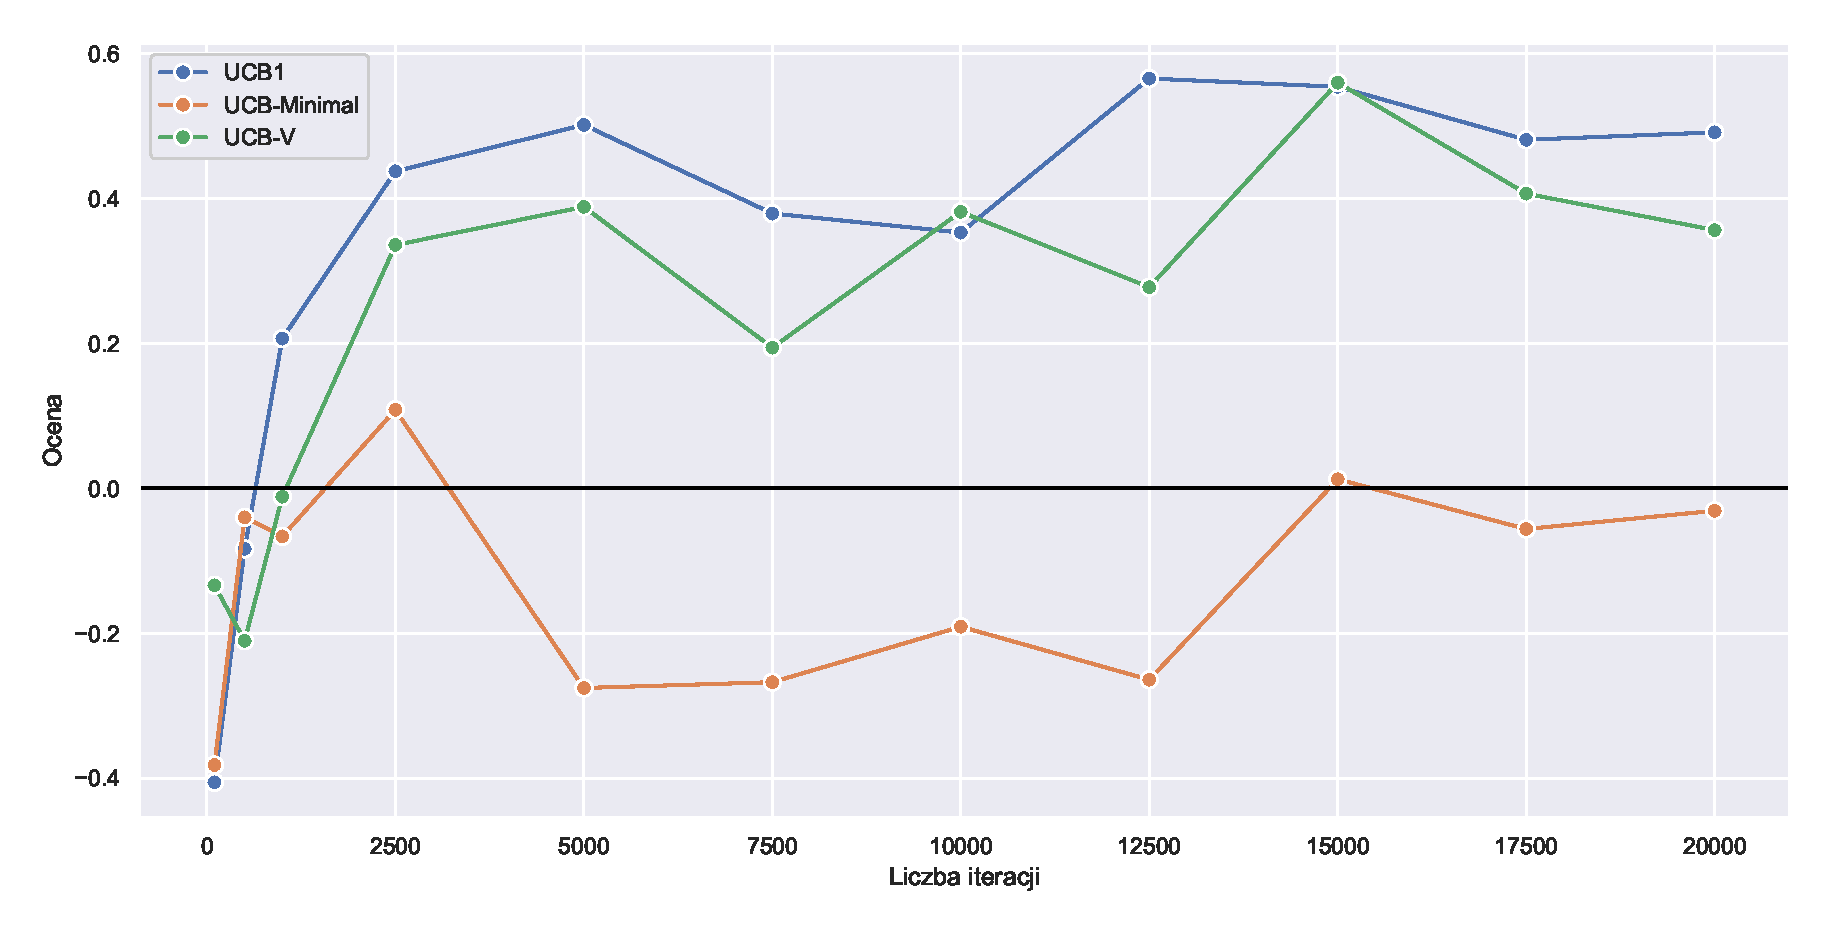
\includegraphics[width=\textwidth]{iterations}
	\caption{Wpływ liczby iteracji na jakość podejmowanych decyzji}
	\label{rys:iterations}
\end{figure}

Wyniki analiz zostały zaprezentowane na wykresie na rysunku \ref{rys:iterations}. Ocena każdego z algorytmów osiąga stosunkowo wysokie wartości przy liczbie iteracji 2500, następnie maleje, by przy liczbie iteracji 15000 osiągnąć najwyższą wartość. Wartym zauważenia jest również fakt, że algorytm UCB-V osiąga relatywnie najlepsze wyniki przy najniższych zakresach iteracji.

\clearpage

\subsection{Najlepszy wariant}
\begin{table}[!h]
	\centering
	\begin{tabular}{|c|c|c|c|c|} \hline
		& UCBV $(1.4, 0.5)$ & UCB1 $(2)$ & UCB1 $(1.41)$ & UCBV $(2, 0.5)$ \\ \hline
		UCBV $(2, 0.5)$ & 0 & 0 & 0 & \cellcolor{lightgray} \\ \hline
		UCB1 $(1.41)$ & 0 & 0 & \cellcolor{lightgray} & \cellcolor{lightgray} \\ \hline
		UCB1 $(2)$ & 0 & \cellcolor{lightgray} & \cellcolor{lightgray} & \cellcolor{lightgray}  \\ \hline
		UCBV $(1.4, 0.5)$ & \cellcolor{lightgray} & \cellcolor{lightgray} & \cellcolor{lightgray} & \cellcolor{lightgray} \\ \hline
	\end{tabular}
	\caption{Ocena najlepszych konfiguracji algorytmów}
	\label{tab:best_variant}
\end{table}

Najlepszy z wariantów zostanie wyłoniony na podstawie rozegrania partii każdy z każdym.

\begin{thebibliography}{20}
	\bibitem[1]{connect4knowledge} Victor Allis, \emph{A Knowledge-based Approach of Connect-Four}, Department of Mathematics and Computer Science Vrije Universiteit Amsterdam, The Netherlands. %https://bit.ly/2SPdKQt
	\bibitem[2]{banditbased} Levente Kocsis, Csaba Szepesvári, \emph{Bandit based Monte-Carlo Planning}, European Conference on Machine Learning, Berlin, Germany, September 18--22, 2006.
	\bibitem[3]{mctsanalysis} Steven James, George Konidaris, Benjamin Rosman, \emph{An Analysis of Monte Carlo Tree Search}, University of the Witwatersrand, Johannesburg, South Africa.
	\bibitem[4]{ucbminimal} Francis Maes, Louis Wehenkel, Damien Ernst, \emph{Automatic Discovery of Ranking Formulas for Playing with Multi-armed Bandits}, European Workshop on Reinforcement Learning, Athens, Greece, September 9--11, 2011.
	\bibitem[5]{tron} Pierre Perick, David L. St-Pierre, Francis Maes, Damien Ernst, \emph{Comparison of Different Selection Strategies in Monte-Carlo Tree Search for the Game of Tron},  IEEE Conference on Computational Intelligence and Games, Granada, Spain, September 12--15, 2012. %https://bit.ly/2y2cvq2
	\bibitem[6]{ucbv} Jean-Yves Audibert, Remi Munos, Csaba Szepesvári, \emph{Tuning Bandit Algorithms in Stochastic Environments}, Algorithmic Learning Theory 18th International Conference, Sendai, Japan, October 1--4, 2007. %https://bit.ly/3d9WcX9
\end{thebibliography}
\end{document}
